\documentclass{report}
\usepackage[showframe=false]{geometry}
\usepackage{titlesec}
\usepackage{amsmath}
\usepackage{graphicx}
\usepackage{float}

\pagenumbering{gobble}

\geometry{tmargin=60pt,bmargin=90pt,lmargin=90pt,
rmargin=90pt}

\titleformat{\chapter}{\normalfont\huge}{\thechapter.}{20pt}{\huge}
\titlespacing*{\chapter} {0pt}{0pt}{10pt}

\begin{document}

\chapter{Section 1}

\section{a}

\par 
Precision and Recall have and inverse relationship given the number  of documents retrieved. Therefore if there was an increase in the number of documents that were returned in the queries then the precision and recall values would change with that increase. precision would most likely drop while recall would most likely increase.

\section{b}

\begin{verbatim}
20 Documents
\end{verbatim}

\begin{equation}
Precision = a/(a+b) = 80\% = a/20
\end{equation}
\begin{equation}
a = 16 
\end{equation}
\begin{equation}
Recall = a/(a+c) = 50\% = 16/(16+c)
\end{equation}
\begin{equation}
c=16
\end{equation}
\begin{equation}
Answer = 16
\end{equation}

\par
relevant documents that are not retrieved by the system  is 16 documents that are relevant but not retrieved

\chapter{Section 2}

\begin{verbatim}
mycorpus <- file.path(".", "CSI58100TextFiles")
library(tm)
library(SnowballC)
docs <- Corpus(DirSource(mycorpus))
docs <- VCorpus(DirSource(mycorpus))
docs <- tm_map(docs, removePunctuation)
docs <- tm_map(docs, tolower)
docs <- tm_map(docs, removeNumbers)
docs <- tm_map(docs, removeWords, stopwords("english"))
docs <- tm_map(docs, stripWhitespace)
docs <- tm_map(docs, PlainTextDocument)
dtm <- DocumentTermMatrix(docs)
tdm <- TermDocumentMatrix(docs)
dim(as.matrix(tdm))
tdm <- as.matrix(tdm)

s11 <- lsa::cosine(as.matrix(tdm)[,1], as.matrix(tdm)[,1])
s12 <- lsa::cosine(as.matrix(tdm)[,1], as.matrix(tdm)[,2])
s13 <- lsa::cosine(as.matrix(tdm)[,1], as.matrix(tdm)[,3])
s14 <- lsa::cosine(as.matrix(tdm)[,1], as.matrix(tdm)[,4])
s15 <- lsa::cosine(as.matrix(tdm)[,1], as.matrix(tdm)[,5])
s16 <- lsa::cosine(as.matrix(tdm)[,1], as.matrix(tdm)[,6])
s17 <- lsa::cosine(as.matrix(tdm)[,1], as.matrix(tdm)[,7])
s18 <- lsa::cosine(as.matrix(tdm)[,1], as.matrix(tdm)[,8])

s21 <- lsa::cosine(as.matrix(tdm)[,2], as.matrix(tdm)[,1])
s22 <- lsa::cosine(as.matrix(tdm)[,2], as.matrix(tdm)[,2])
s23 <- lsa::cosine(as.matrix(tdm)[,2], as.matrix(tdm)[,3])
s24 <- lsa::cosine(as.matrix(tdm)[,2], as.matrix(tdm)[,4])
s25 <- lsa::cosine(as.matrix(tdm)[,2], as.matrix(tdm)[,5])
s26 <- lsa::cosine(as.matrix(tdm)[,2], as.matrix(tdm)[,6])
s27 <- lsa::cosine(as.matrix(tdm)[,2], as.matrix(tdm)[,7])
s28 <- lsa::cosine(as.matrix(tdm)[,2], as.matrix(tdm)[,8])

s31 <- lsa::cosine(as.matrix(tdm)[,3], as.matrix(tdm)[,1])
s32 <- lsa::cosine(as.matrix(tdm)[,3], as.matrix(tdm)[,2])
s33 <- lsa::cosine(as.matrix(tdm)[,3], as.matrix(tdm)[,3])
s34 <- lsa::cosine(as.matrix(tdm)[,3], as.matrix(tdm)[,4])
s35 <- lsa::cosine(as.matrix(tdm)[,3], as.matrix(tdm)[,5])
s36 <- lsa::cosine(as.matrix(tdm)[,3], as.matrix(tdm)[,6])
s37 <- lsa::cosine(as.matrix(tdm)[,3], as.matrix(tdm)[,7])
s38 <- lsa::cosine(as.matrix(tdm)[,3], as.matrix(tdm)[,8])

s41 <- lsa::cosine(as.matrix(tdm)[,4], as.matrix(tdm)[,1])
s42 <- lsa::cosine(as.matrix(tdm)[,4], as.matrix(tdm)[,2])
s43 <- lsa::cosine(as.matrix(tdm)[,4], as.matrix(tdm)[,3])
s44 <- lsa::cosine(as.matrix(tdm)[,4], as.matrix(tdm)[,4])
s45 <- lsa::cosine(as.matrix(tdm)[,4], as.matrix(tdm)[,5])
s46 <- lsa::cosine(as.matrix(tdm)[,4], as.matrix(tdm)[,6])
s47 <- lsa::cosine(as.matrix(tdm)[,4], as.matrix(tdm)[,7])
s48 <- lsa::cosine(as.matrix(tdm)[,4], as.matrix(tdm)[,8])

s51 <- lsa::cosine(as.matrix(tdm)[,5], as.matrix(tdm)[,1])
s52 <- lsa::cosine(as.matrix(tdm)[,5], as.matrix(tdm)[,2])
s53 <- lsa::cosine(as.matrix(tdm)[,5], as.matrix(tdm)[,3])
s54 <- lsa::cosine(as.matrix(tdm)[,5], as.matrix(tdm)[,4])
s55 <- lsa::cosine(as.matrix(tdm)[,5], as.matrix(tdm)[,5])
s56 <- lsa::cosine(as.matrix(tdm)[,5], as.matrix(tdm)[,6])
s57 <- lsa::cosine(as.matrix(tdm)[,5], as.matrix(tdm)[,7])
s58 <- lsa::cosine(as.matrix(tdm)[,5], as.matrix(tdm)[,8])

s61 <- lsa::cosine(as.matrix(tdm)[,6], as.matrix(tdm)[,1])
s62 <- lsa::cosine(as.matrix(tdm)[,6], as.matrix(tdm)[,2])
s63 <- lsa::cosine(as.matrix(tdm)[,6], as.matrix(tdm)[,3])
s64 <- lsa::cosine(as.matrix(tdm)[,6], as.matrix(tdm)[,4])
s65 <- lsa::cosine(as.matrix(tdm)[,6], as.matrix(tdm)[,5])
s66 <- lsa::cosine(as.matrix(tdm)[,6], as.matrix(tdm)[,6])
s67 <- lsa::cosine(as.matrix(tdm)[,6], as.matrix(tdm)[,7])
s68 <- lsa::cosine(as.matrix(tdm)[,6], as.matrix(tdm)[,8])

s71 <- lsa::cosine(as.matrix(tdm)[,7], as.matrix(tdm)[,1])
s72 <- lsa::cosine(as.matrix(tdm)[,7], as.matrix(tdm)[,2])
s73 <- lsa::cosine(as.matrix(tdm)[,7], as.matrix(tdm)[,3])
s74 <- lsa::cosine(as.matrix(tdm)[,7], as.matrix(tdm)[,4])
s75 <- lsa::cosine(as.matrix(tdm)[,7], as.matrix(tdm)[,5])
s76 <- lsa::cosine(as.matrix(tdm)[,7], as.matrix(tdm)[,6])
s77 <- lsa::cosine(as.matrix(tdm)[,7], as.matrix(tdm)[,7])
s78 <- lsa::cosine(as.matrix(tdm)[,7], as.matrix(tdm)[,8])

s81 <- lsa::cosine(as.matrix(tdm)[,8], as.matrix(tdm)[,1])
s82 <- lsa::cosine(as.matrix(tdm)[,8], as.matrix(tdm)[,2])
s83 <- lsa::cosine(as.matrix(tdm)[,8], as.matrix(tdm)[,3])
s84 <- lsa::cosine(as.matrix(tdm)[,8], as.matrix(tdm)[,4])
s85 <- lsa::cosine(as.matrix(tdm)[,8], as.matrix(tdm)[,5])
s86 <- lsa::cosine(as.matrix(tdm)[,8], as.matrix(tdm)[,6])
s87 <- lsa::cosine(as.matrix(tdm)[,8], as.matrix(tdm)[,7])
s88 <- lsa::cosine(as.matrix(tdm)[,8], as.matrix(tdm)[,8])

matrix(c(s11, s12, s13, s14, s15, s16, s17, s18, s21, s22, s23, s24, s25, s26, s27, s28, s31, s32, s33, s34, s35, s36, s37, s38, s41, s42, s43, s44, s45, s46, s47, s48, s51, s52, s53, s54, s55, s56, s57, s58, s61, s62, s63, s64, s65, s66, s67, s68, s71, s72, s73, s74, s75, s76, s77, s78, s81, s82, s83, s84, s85, s86, s87, s88), 8, 8)
\end{verbatim}

\[
  dim <- 
  \begin{bmatrix}
    893 & x & 8
  \end{bmatrix}
\]

Cosine Similarity = 
\[
  \begin{bmatrix}
    1.00000000 & 0.08532917 & 0.11599068 & 0.08782695 & 0.02563073 & 0.13632185 & 0.09823684 & 0.05459680 \\
    0.08532917 & 1.00000000 & 0.05884278 & 0.08823251 & 0.04494386 & 0.07406946 & 0.05637591 & 0.06718335 \\
    0.11599068 & 0.05884278 & 1.00000000 & 0.02797851 & 0.02561578 & 0.07138330 & 0.02998938 & 0.04135449 \\
    0.08782695 & 0.08823251 & 0.02797851 & 1.00000000 & 0.13813590 & 0.14005778 & 0.16655658 & 0.05186247 \\
    0.02563073 & 0.04494386 & 0.02561578 & 0.13813590 & 1.00000000 & 0.07416198 & 0.05017452 & 0.02354355 \\
    0.13632185 & 0.07406946 & 0.07138330 & 0.14005778 & 0.07416198 & 1.00000000 & 0.07517257 & 0.03325783 \\
    0.09823684 & 0.05637591 & 0.02998938 & 0.16655658 & 0.05017452 & 0.07517257 & 1.00000000 & 0.02531328 \\
    0.05459680 & 0.06718335 & 0.04135449 & 0.05186247 & 0.02354355 & 0.03325783 & 0.02531328 & 1.00000000
  \end{bmatrix}
\]


\chapter{Section 3}

\begin{verbatim}
dtm_tfidf <- DocumentTermMatrix(docs, control = list(weighting = weightTfIdf))
dtm_tfidf <- as.matrix(dtm_tfidf)
dim(dtm_tfidf)

s11 <- lsa::cosine(dtm_tfidf[1,], dtm_tfidf[1,])
s12 <- lsa::cosine(dtm_tfidf[1,], dtm_tfidf[2,])
s13 <- lsa::cosine(dtm_tfidf[1,], dtm_tfidf[3,])
s14 <- lsa::cosine(dtm_tfidf[1,], dtm_tfidf[4,])
s15 <- lsa::cosine(dtm_tfidf[1,], dtm_tfidf[5,])
s16 <- lsa::cosine(dtm_tfidf[1,], dtm_tfidf[6,])
s17 <- lsa::cosine(dtm_tfidf[1,], dtm_tfidf[7,])
s18 <- lsa::cosine(dtm_tfidf[1,], dtm_tfidf[8,])

s21 <- lsa::cosine(dtm_tfidf[2,], dtm_tfidf[1,])
s22 <- lsa::cosine(dtm_tfidf[2,], dtm_tfidf[2,])
s23 <- lsa::cosine(dtm_tfidf[2,], dtm_tfidf[3,])
s24 <- lsa::cosine(dtm_tfidf[2,], dtm_tfidf[4,])
s25 <- lsa::cosine(dtm_tfidf[2,], dtm_tfidf[5,])
s26 <- lsa::cosine(dtm_tfidf[2,], dtm_tfidf[6,])
s27 <- lsa::cosine(dtm_tfidf[2,], dtm_tfidf[7,])
s28 <- lsa::cosine(dtm_tfidf[2,], dtm_tfidf[8,])

s31 <- lsa::cosine(dtm_tfidf[3,], dtm_tfidf[1,])
s32 <- lsa::cosine(dtm_tfidf[3,], dtm_tfidf[2,])
s33 <- lsa::cosine(dtm_tfidf[3,], dtm_tfidf[3,])
s34 <- lsa::cosine(dtm_tfidf[3,], dtm_tfidf[4,])
s35 <- lsa::cosine(dtm_tfidf[3,], dtm_tfidf[5,])
s36 <- lsa::cosine(dtm_tfidf[3,], dtm_tfidf[6,])
s37 <- lsa::cosine(dtm_tfidf[3,], dtm_tfidf[7,])
s38 <- lsa::cosine(dtm_tfidf[3,], dtm_tfidf[8,])

s41 <- lsa::cosine(dtm_tfidf[4,], dtm_tfidf[1,])
s42 <- lsa::cosine(dtm_tfidf[4,], dtm_tfidf[2,])
s43 <- lsa::cosine(dtm_tfidf[4,], dtm_tfidf[3,])
s44 <- lsa::cosine(dtm_tfidf[4,], dtm_tfidf[4,])
s45 <- lsa::cosine(dtm_tfidf[4,], dtm_tfidf[5,])
s46 <- lsa::cosine(dtm_tfidf[4,], dtm_tfidf[6,])
s47 <- lsa::cosine(dtm_tfidf[4,], dtm_tfidf[7,])
s48 <- lsa::cosine(dtm_tfidf[4,], dtm_tfidf[8,])

s51 <- lsa::cosine(dtm_tfidf[5,], dtm_tfidf[1,])
s52 <- lsa::cosine(dtm_tfidf[5,], dtm_tfidf[2,])
s53 <- lsa::cosine(dtm_tfidf[5,], dtm_tfidf[3,])
s54 <- lsa::cosine(dtm_tfidf[5,], dtm_tfidf[4,])
s55 <- lsa::cosine(dtm_tfidf[5,], dtm_tfidf[5,])
s56 <- lsa::cosine(dtm_tfidf[5,], dtm_tfidf[6,])
s57 <- lsa::cosine(dtm_tfidf[5,], dtm_tfidf[7,])
s58 <- lsa::cosine(dtm_tfidf[5,], dtm_tfidf[8,])

s61 <- lsa::cosine(dtm_tfidf[6,], dtm_tfidf[1,])
s62 <- lsa::cosine(dtm_tfidf[6,], dtm_tfidf[2,])
s63 <- lsa::cosine(dtm_tfidf[6,], dtm_tfidf[3,])
s64 <- lsa::cosine(dtm_tfidf[6,], dtm_tfidf[4,])
s65 <- lsa::cosine(dtm_tfidf[6,], dtm_tfidf[5,])
s66 <- lsa::cosine(dtm_tfidf[6,], dtm_tfidf[6,])
s67 <- lsa::cosine(dtm_tfidf[6,], dtm_tfidf[7,])
s68 <- lsa::cosine(dtm_tfidf[6,], dtm_tfidf[8,])

s71 <- lsa::cosine(dtm_tfidf[7,], dtm_tfidf[1,])
s72 <- lsa::cosine(dtm_tfidf[7,], dtm_tfidf[2,])
s73 <- lsa::cosine(dtm_tfidf[7,], dtm_tfidf[3,])
s74 <- lsa::cosine(dtm_tfidf[7,], dtm_tfidf[4,])
s75 <- lsa::cosine(dtm_tfidf[7,], dtm_tfidf[5,])
s76 <- lsa::cosine(dtm_tfidf[7,], dtm_tfidf[6,])
s77 <- lsa::cosine(dtm_tfidf[7,], dtm_tfidf[7,])
s78 <- lsa::cosine(dtm_tfidf[7,], dtm_tfidf[8,])

s81 <- lsa::cosine(dtm_tfidf[8,], dtm_tfidf[1,])
s82 <- lsa::cosine(dtm_tfidf[8,], dtm_tfidf[2,])
s83 <- lsa::cosine(dtm_tfidf[8,], dtm_tfidf[3,])
s84 <- lsa::cosine(dtm_tfidf[8,], dtm_tfidf[4,])
s85 <- lsa::cosine(dtm_tfidf[8,], dtm_tfidf[5,])
s86 <- lsa::cosine(dtm_tfidf[8,], dtm_tfidf[6,])
s87 <- lsa::cosine(dtm_tfidf[8,], dtm_tfidf[7,])
s88 <- lsa::cosine(dtm_tfidf[8,], dtm_tfidf[8,])
\end{verbatim}

\[
  dim <- 
  \begin{bmatrix}
    8 & x & 893
  \end{bmatrix}
\]

Cosine Similarity = 
\[
  \begin{bmatrix}
  1.000000000 & 0.01299370 & 0.037984165 & 0.03534426 & 0.006695362 & 0.028322122 & 0.024298992 & 0.021710345 \\
  0.012993697 & 1.00000000 & 0.012926329 & 0.02864772 & 0.012736616 & 0.013470094 & 0.016013411 & 0.018054686 \\
  0.037984165 & 0.01292633 & 1.000000000 & 0.01061389 & 0.008382378 & 0.015091381 & 0.005744139 & 0.006750641 \\
  0.035344261 & 0.02864772 & 0.010613894 & 1.00000000 & 0.058684798 & 0.050313417 & 0.058260906 & 0.024900624 \\
  0.006695362 & 0.01273662 & 0.008382378 & 0.05868480 & 1.000000000 & 0.018163552 & 0.020138165 & 0.011408900 \\
  0.028322122 & 0.01347009 & 0.015091381 & 0.05031342 & 0.018163552 & 1.000000000 & 0.016925851 & 0.007200809 \\
  0.024298992 & 0.01601341 & 0.005744139 & 0.05826091 & 0.020138165 & 0.016925851 & 1.000000000 & 0.008400867 \\
  0.021710345 & 0.01805469 & 0.006750641 & 0.02490062 & 0.011408900 & 0.007200809 & 0.025313276 & 1.000000000
  \end{bmatrix}
\]


\chapter{Section 4}

\section{i}

\begin{verbatim}
records <- t(matrix(c(1,0, 1, 0,1, 1, 0,-1, 1, 0,0, 2, 0,2, 2, 0,-2, 2, -2,0, 2), 3, 7))
plot(records[,0:2], pch=21, bg=c("green", "blue")[records[,3]])
segments(1.1, 1.5, -1, 1.5, col= 'red')
segments(-1, .5, -1, 1.5, col= 'red')
segments(.5, .5, -1, .5, col= 'red')
segments(.5, -.5, .5, .5, col= 'red')
segments(.5, -.5, -1, -.5, col= 'red')
segments(-1, -.5, -1, -1.5, col= 'red')
segments(-1, -1.5, 1.1, -1.5, col= 'red')
\end{verbatim}

\[
  records <- 
  \begin{bmatrix}
    1 & 0 & 1 \\
    0 & 1 & 1 \\
    0 & -1 & 1 \\
    0 & 0 & 2 \\
    0 & 2 & 2 \\
    0 & -2 & 2 \\
    -2 & 0 & 2
  \end{bmatrix}
\]

\begin{figure}[H]
	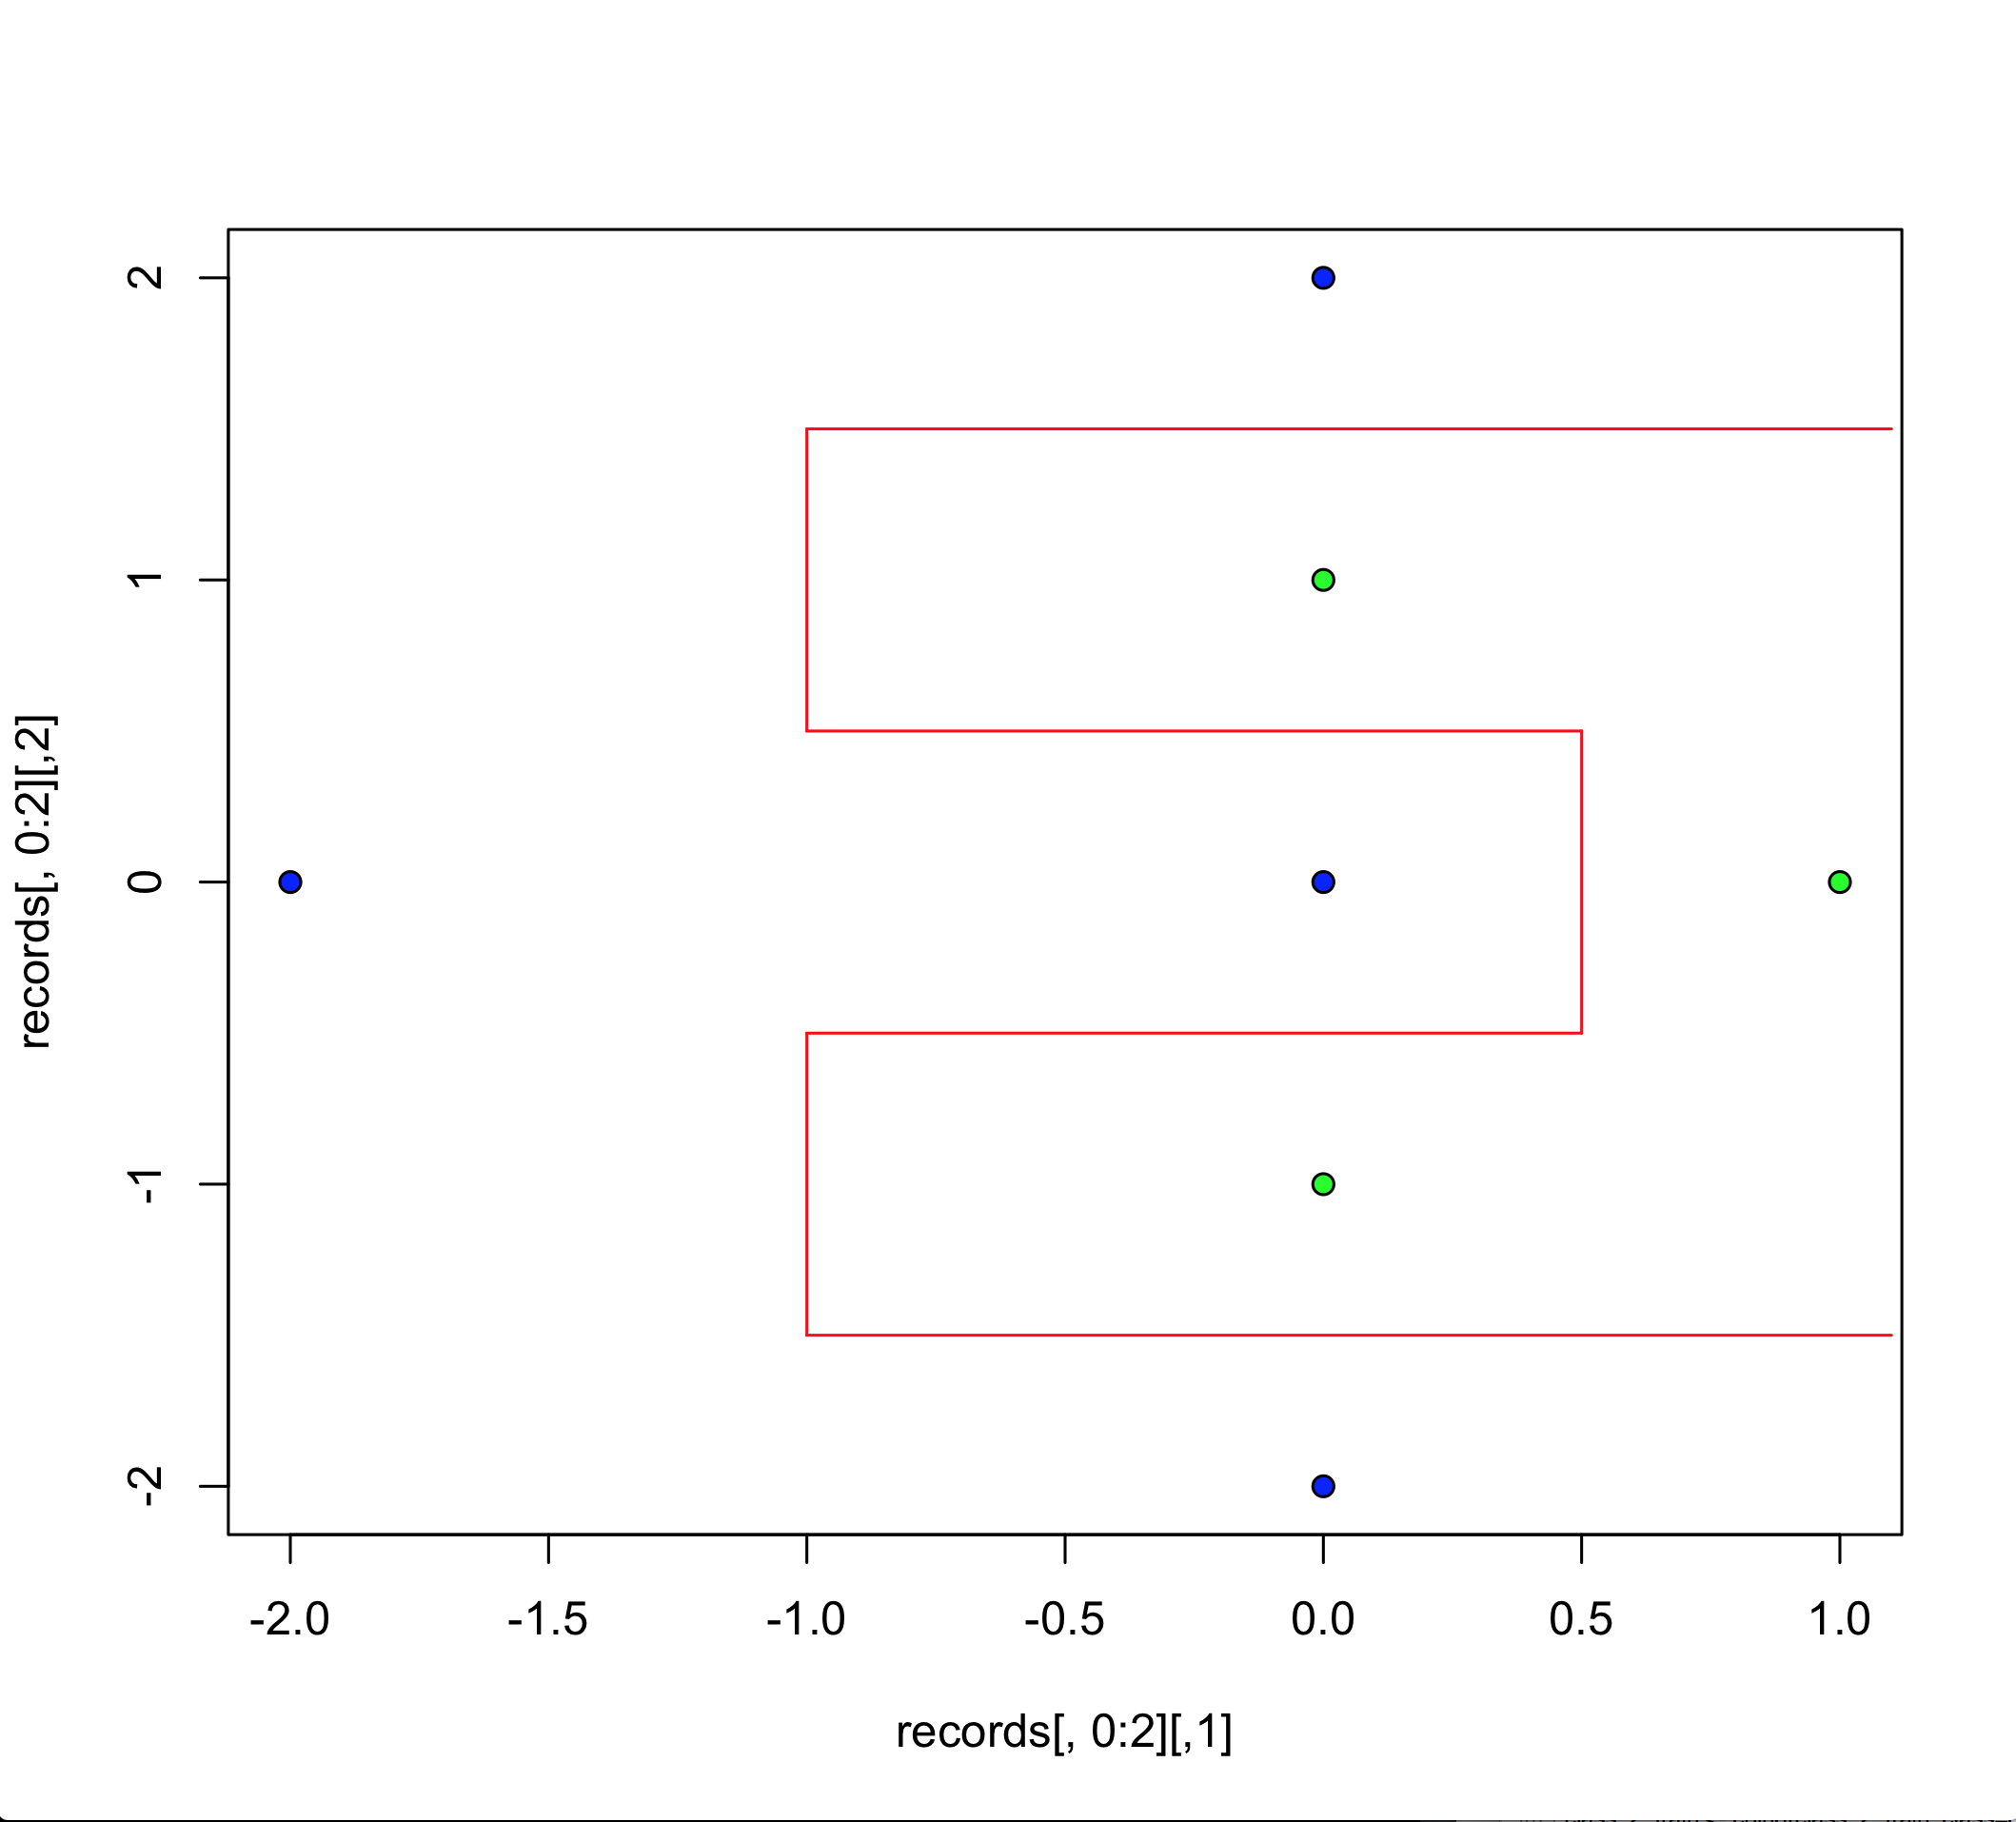
\includegraphics[width=\linewidth]{1-NN_decision_boundary.png}
	 \caption{Sketch Decision Boundary Due To 1-NN Rule}
\end{figure}

\section{ii}

\begin{verbatim}
records_class_1 <- t(matrix(c(1,0, 0,1, 0,-1), 2, 3))
records_class_2 <- t(matrix(c(0,0, 0,2, 0,-2, -2,0), 2, 4))
class_1_mean <- colMeans(records_class_1)
class_2_mean <- colMeans(records_class_2)
plot(records[,0:2], pch=21, bg=c("green", "blue")[records[,3]])
points(x=class_1_mean[1], y=class_1_mean[2], pch=22, bg="green")
points(x=class_2_mean[1], y=class_2_mean[2], pch=22, bg="blue")
means <- t(matrix(c(class_1_mean, class_2_mean), 2,2))
segments(colMeans(means)[1], 2.2, colMeans(means)[1], -2.2, col= 'red')
\end{verbatim}

\[
  records\_class\_1 <- 
  \begin{bmatrix}
    1 & 0 \\
    0 & 1 \\
    0 & -1
  \end{bmatrix}
\]

\[
  records\_class\_2 <- 
  \begin{bmatrix}
    0 & 0 \\
    0 & 2 \\
    0 & -2 \\
    -2 & 0
  \end{bmatrix}
\]

\[
  class\_1\_mean <- 
  \begin{bmatrix}
    0.3333333 & 0.0
  \end{bmatrix}
\]

\[
  class\_2\_mean <- 
  \begin{bmatrix}
    -0.5 & 0.0
  \end{bmatrix}
\]

\[
  means <- 
  \begin{bmatrix}
     0.3333333 & 0.0 \\
    -0.5 & 0.0
  \end{bmatrix}
\]

\[
  line <- 
  \begin{bmatrix}
     x = -0.08333333 \\
     y = 0.0
   \end{bmatrix}
\]

\begin{figure}[H]
	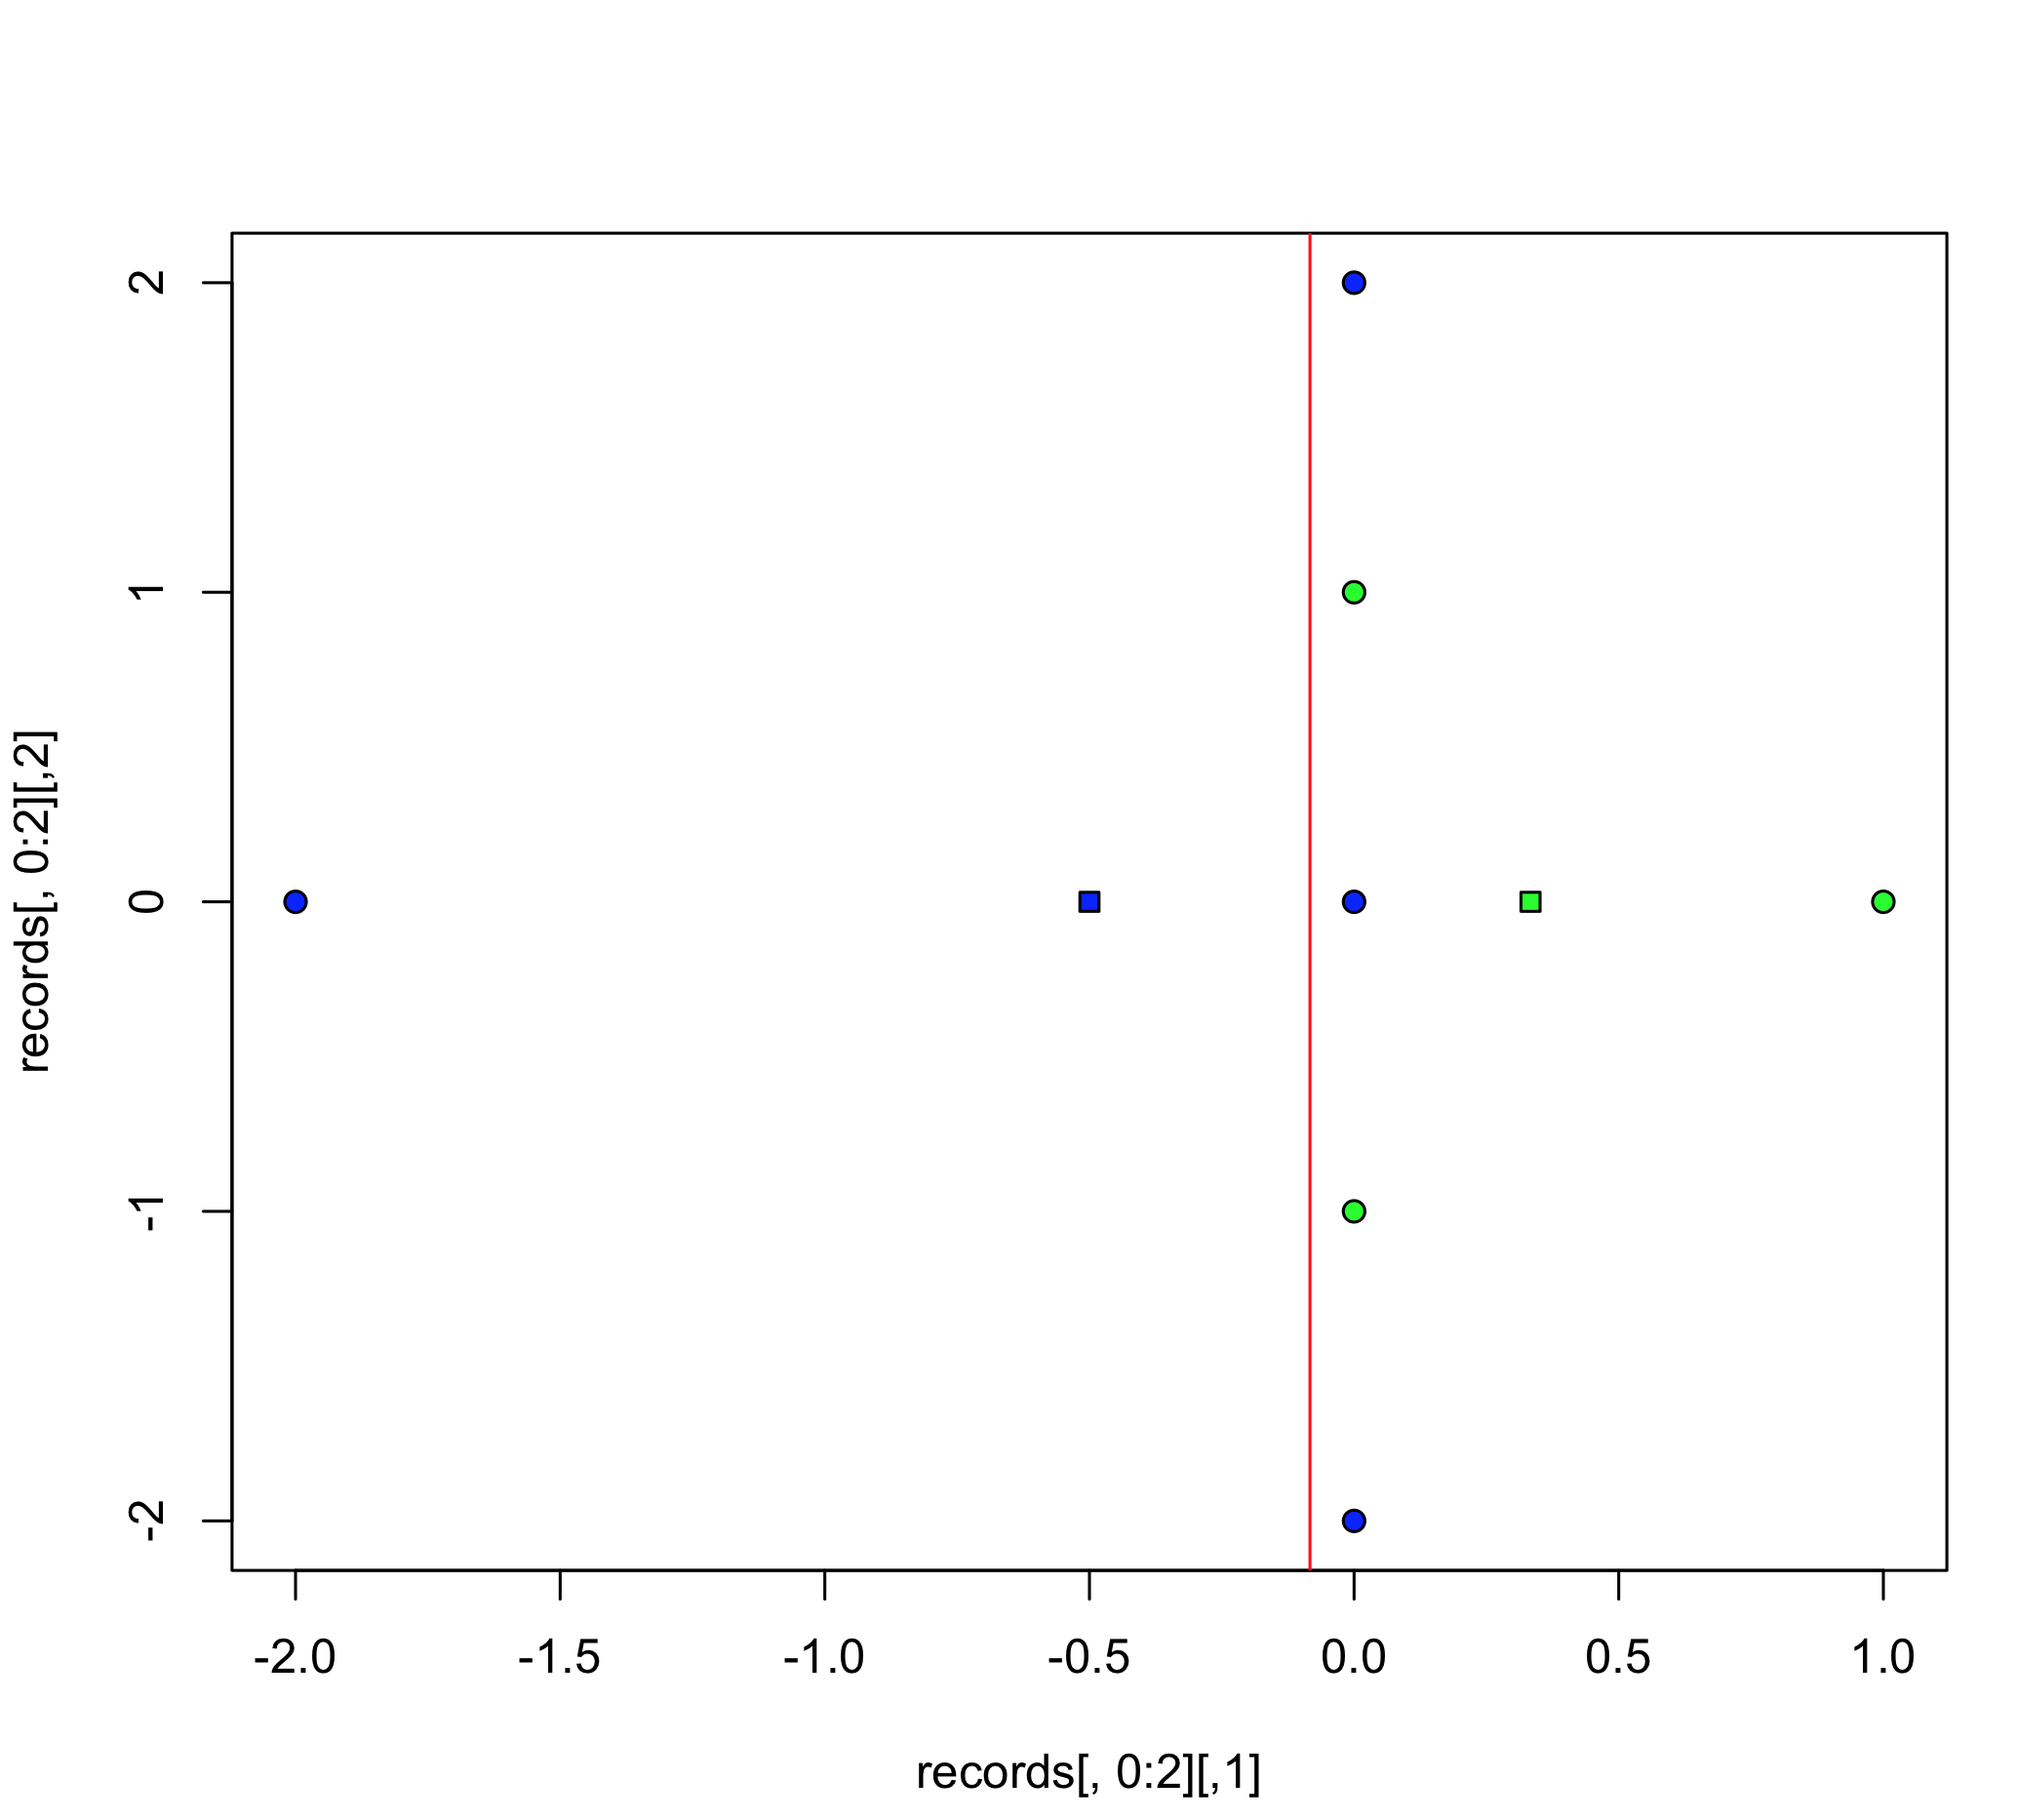
\includegraphics[width=\linewidth]{Minimum_Distance_Decision_Boundary.png}
	 \caption{Sample Means Sketch Minimum Distance Decision Boundary.}
\end{figure}

\chapter{Section 5}


\begin{verbatim}
library(readxl)
library("car")
library("class")

wheatData <- read_excel("wheatdata.xlsx")

class_1_train <- wheatData[0:25,2:7]
class_2_train <- wheatData[0:25,8:13]
class_1_test <- wheatData[26:27,2:7]
class_2_test <- wheatData[26:27,8:13]
class_1_train <- cbind(class_1_train, class=c(1,1,1,1,1,1,1,1,1,1,1,1,1,1,1,1,1,1,1,1,1,1,1,1,1))
class_2_train <- cbind(class_2_train, class=c(2,2,2,2,2,2,2,2,2,2,2,2,2,2,2,2,2,2,2,2,2,2,2,2,2))
class_train <- rbind(as.matrix(class_1_train), as.matrix(class_2_train))
class_test <- rbind(as.matrix(class_1_test), as.matrix(class_2_test))

scatterplotMatrix(class_train[,0:6], smoother="FALSE", reg.line="FALSE")
class_train <- data.frame(class_train)
sapply(class_train[0:6],mean)
sapply(class_train[0:6],sd)
\end{verbatim}

\[
  class\_1\_test <- 
  \begin{bmatrix}
	92.05 & 212 & 9.81 & 13.1 & 304 & 13.9 \\
	76.80 & 193 & 9.80 & 13.1 & 288 & 13.4
   \end{bmatrix}
\]

\[
  class\_2\_test <- 
  \begin{bmatrix}
	80.45  & 172 & 11.32 & 14.3 & 306 & 18.7 \\
	83.75 & 202 & 10.38 & 13.4 & 343 & 13.8
   \end{bmatrix}
\]

\[
  mean <- 
  \begin{bmatrix}
	78.7240 & 169.4600 & 10.1406 & 12.9160 & 335.8200 & 14.7260
   \end{bmatrix}
\]

\[
  sd <- 
  \begin{bmatrix}
	6.8176110 & 21.9333034 & 0.6163633 & 0.8723321 & 46.1424989 & 2.1222639
   \end{bmatrix}
\]

\begin{figure}[H]
	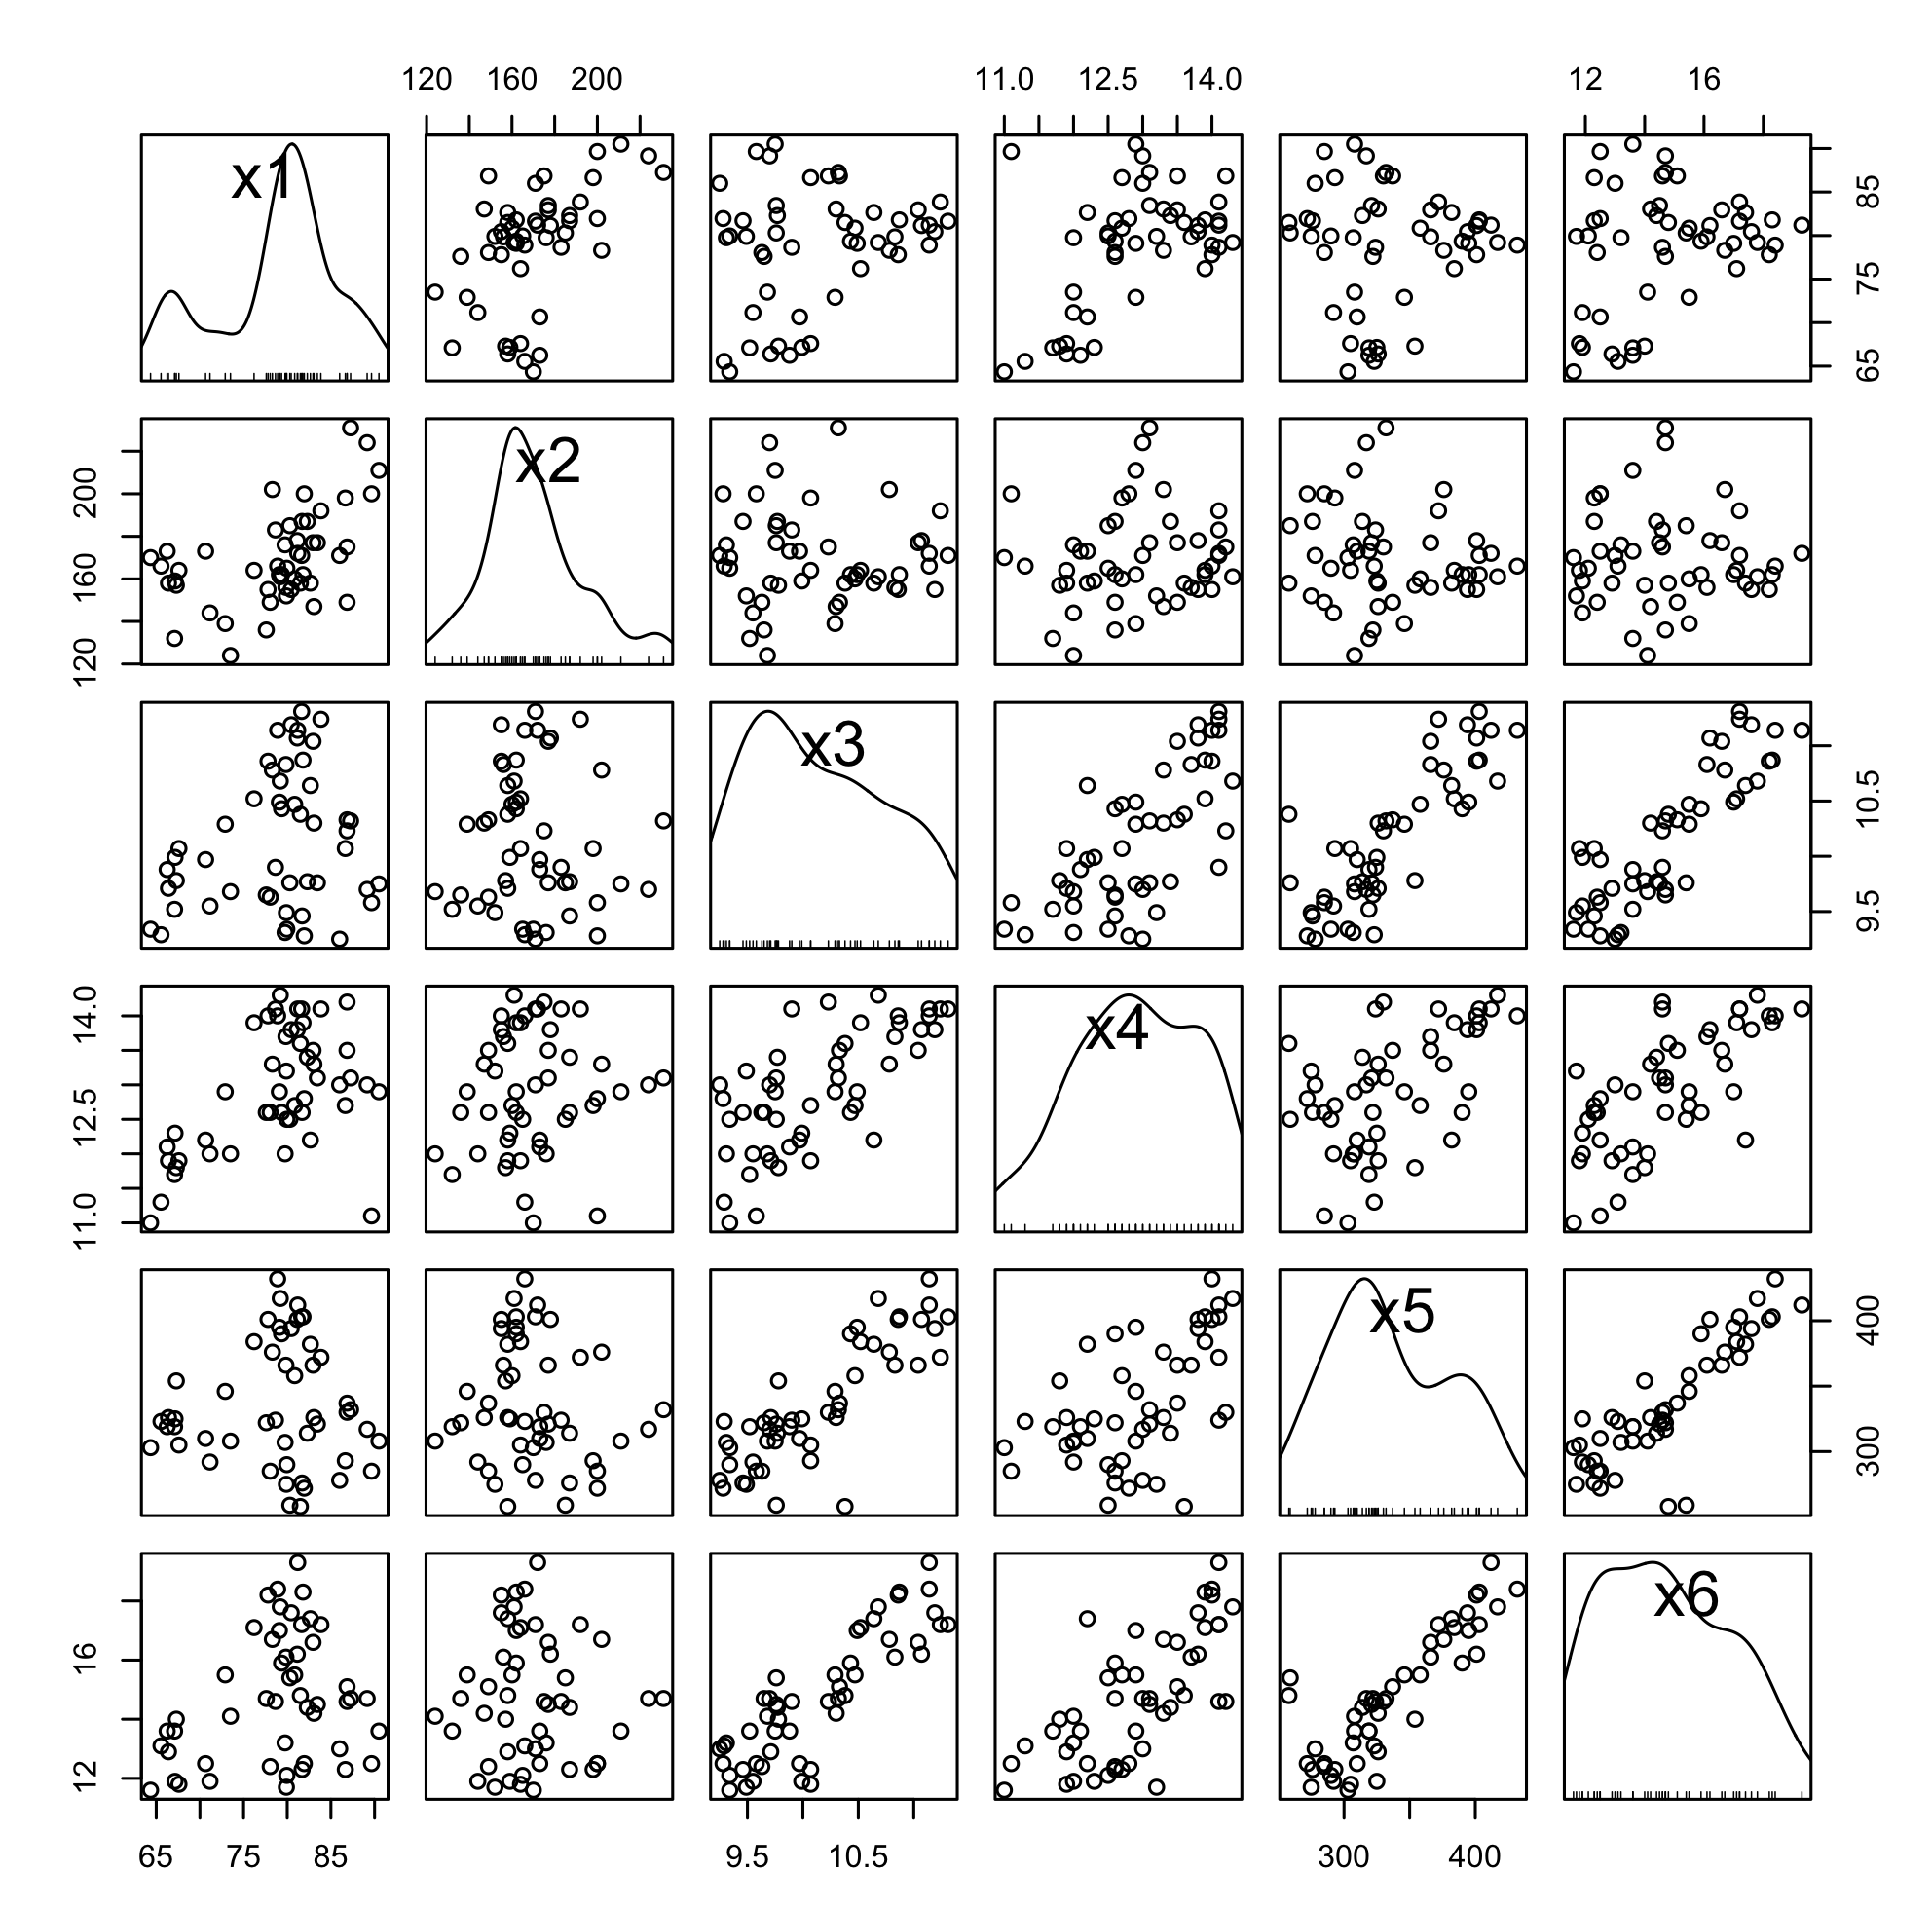
\includegraphics[width=\linewidth]{wheatdata_features.png}
	 \caption{Wheat Data Features}
\end{figure}

\section{K-NN 1-NN}

\begin{verbatim}
c1 <- factor(c(rep(1,25), rep(2,25)))
knn(class_train[,0:6], class_test, c1, k=1)
\end{verbatim}

\[
  training\_set\_outcome <- 
  \begin{bmatrix}
	1 & 1 & 1 & 1
   \end{bmatrix}
\]

\[
  class\_1\_test\_1 <- 
  \begin{bmatrix}
	92.05 & 212 & 9.81 & 13.1 & 304 & 13.9
   \end{bmatrix}
\]

\[
  class\_1\_test\_1\_nearest\_neighbor <- 
  \begin{bmatrix}
	90.50 & 211 & 9.75 & 12.90 & 308 & 13.60
   \end{bmatrix}
\]

\[
  class\_1\_test\_2 <- 
  \begin{bmatrix}
	76.80 & 193 & 9.80 & 13.1 & 288 & 13.4
   \end{bmatrix}
\]

\[
  class\_1\_test\_2\_nearest\_neighbor <- 
  \begin{bmatrix}
	86.65 & 198 & 10.07 & 12.70 & 293 & 12.30
   \end{bmatrix}
\]

\[
  class\_2\_test\_1 <- 
  \begin{bmatrix}
	80.45  & 172 & 11.32 & 14.3 & 306 & 18.7
   \end{bmatrix}
\]

\[
  class\_2\_test\_1\_nearest\_neighbor <- 
  \begin{bmatrix}
	79.75 & 176 & 9.31 & 12.00 & 307 & 13.20
   \end{bmatrix}
\]

\[
  class\_2\_test\_2 <- 
  \begin{bmatrix}
	83.75 & 202 & 10.38 & 13.4 & 343 & 13.8
   \end{bmatrix}
\]

\[
  class\_2\_test\_2\_nearest\_neighbor <- 
  \begin{bmatrix}
  	78.65 & 183 & 9.90 & 14.10 & 324 & 14.60
   \end{bmatrix}
\]

\section{Na�ve Bayes Classifier}

\begin{verbatim}
library("caret")
x = class_train[,-7]
y = class_train[,7]
model = train(x, as.factor(y), 'nb', trControl=trainControl(method='cv',number=10))
predict(model$finalModel, class_test)
table(predict(model$finalModel, class_test)$class, c(1,1,2,2))
\end{verbatim}

\[
  prediction <- 
  \begin{bmatrix}
  1 & 2 \\
  	0.9999106444 & 8.935565e-05 \\
	0.9919994992 & 8.000501e-03 \\
	0.0000149507 & 9.999850e-01 \\
	0.9286506398 & 7.134936e-02
   \end{bmatrix}
\]

\[
  training\_set\_outcome <- 
  \begin{bmatrix}
	1 & 1 & 2 & 1
   \end{bmatrix}
\]

\[
  error table <- 
  \begin{bmatrix}
  	   & & 1 & 2 \\
	-- & -- & -- & --\\
	1 & | & 2 & 1 \\
	2 & | & 0 & 1
   \end{bmatrix}
\]

\end{document}







































